\documentclass{article}

\title{WMC Junior Finals Proof Questions - Set 3}
\author{Fredric Gregory King Chung}
\date{\today}

\usepackage{amssymb}
\usepackage{amsfonts}
\usepackage{amsmath}
\usepackage{graphicx}
\usepackage{float}
\usepackage[margin=1in]{geometry}

\begin{document}
\maketitle

\section{The Binomial Theorem by Counting}

\noindent\textbf{Problem 1a.} For any $n, k \in \mathbb{N}_0$ where $k \leq n$, state the number of copies of $x^k$ which result from FOILing out $(1+x)^n$. Hence, show that the coefficient of $x^k$ in the expansion of $(1+x)^n$ is $\binom{n}{k}$.

\bigskip

\noindent\textbf{Solution 1a.}
\[
    (1+x)^n = \underbrace{(1+x)(1+x)\cdots(1+x)}_{n \text{ copies}}.
\]
To get $x^k$, one must select $k$ $x$'s and $n-k$ $1$'s from the $n$ copies of $1+x$. There are $\binom{n}{k}$ ways to do this, so $x^k$ occurs $\binom{n}{k}$ times. Hence, the coefficient of $x^k$ is $\binom{n}{k}$. $\qquad \square$

\bigskip

\noindent\textbf{Problem 1b.} Show that
\[
    \binom{n}{k} = \frac{n(n-1)\cdots(n-k+1)}{k!}
\]
for any $n, k \in \mathbb{N}_0$ where $k \leq n$.

\bigskip

\noindent\textbf{Solution 1b.}
\[
    \binom{n}{k}
    = \frac{n!}{k!\,(n-k)!}
    = \frac{n(n-1)\cdots(n-k+1) \cdot (n-k)!}{k!\,(n-k)!}
    = \boxed{\frac{n(n-1)\cdots(n-k+1)}{k!}}
\]

\section{Negative Integer Exponents via Stars and Bars}

\noindent\textbf{Problem 2.} Show that
\[
    (1+x)^n = \sum_{k=0}^{\infty} \frac{n(n-1)\cdots(n-k+1)}{k!}\, x^k
\]
for $n \in \mathbb{Z}^-$ and $|x| < 1$.

\bigskip

\noindent\textbf{Solution 2.} The key idea is to notice that $\frac{1}{1-x}$ can be expanded out into a geometric series, which can be FOILed and inspected combinatorially.

\medskip

\noindent Because
\[
    \frac{1}{1-x} = 1 + x + x^2 + \cdots
\]
(the RHS converges, as $|x| < 1$), we look at $(1-x)^n$ first. Then,
\begin{align*}
    (1-x)^n &= \left(\frac{1}{1-x}\right)^{-n} \\
            &= \left(1 + x + x^2 + \cdots\right)^{-n} \\
            &= \underbrace{\left(1 + x + x^2 + \cdots\right) \cdots \left(1 + x + x^2 + \cdots\right)}_{-n \text{ copies}}.
\end{align*}
The coefficient of $x^k$ here is the number of times it occurs. Consider which powers of $x$ we need to get from each of $-n$ copies of $1 + x + x^2 + \cdots$ to get $x^k$. The number of ways we can get $x^k$ is the number of ways to write the integer $k$ as an ordered sum of $-n$ nonnegative integer terms (the weak compositions of $k$ into $-n$ parts), as each term corresponds to the power of $x$ chosen from $\left(1 + x + x^2 + \cdots\right)$.

\medskip

\noindent The number of such sums can be found using Stars and Bars: $k$ stars and $-n$ groups, so $-n-1$ bars. The coefficient of $x^k$ is thus
\begin{align*}
    \binom{(-n-1)+k}{k} &= \binom{k-n-1}{k} \\
                        &= \frac{(k-n-1)!}{k!\,(-n-1)!} \\
                        &= \frac{(k-n-1)(k-n-2)\cdots(-n)}{k!} \\
                        &= \frac{n(n-1)\cdots(n-k+1)}{k!} \cdot (-1)^k.
\end{align*}
Hence,
\begin{align*}
    (1+x)^n &= \left[1 - (-x)\right]^n \\
            &= \sum_{k=0}^{\infty} \frac{n(n-1)\cdots(n-k+1)}{k!} \cdot (-1)^k (-x)^k \\
            &= \sum_{k=0}^{\infty} \frac{n(n-1)\cdots(n-k+1)}{k!}\, x^k,
\end{align*}
as desired. $\qquad \square$

\section{The Extended Binomial Theorem via Taylor Series}

\noindent\textbf{Problem 3a.} \textit{(Probably Senior Finals level.)} Let $f(x) = (1+x)^n$, where $n \notin \mathbb{N}_0$. Find the Taylor Series of $f$ centered on $x = 0$. (\textbf{Hint:} This happens to give the Extended Binomial Theorem.)

\bigskip

\noindent\textbf{Solution 3a.} Let $P(m)$ be the proposition that
\[
    f^{(m)}(x) = \underset{1}{n}\,\underset{2}{(n-1)}\,\underset{\cdots}{\cdots}\,\underset{m}{(n-m+1)}\,(1+x)^{n-m}
\]
for $m \in \mathbb{Z}^+$. We can prove $P(m)$ holds for all $m \in \mathbb{Z}^+$ using induction.

\medskip

\noindent Our base case is $P(1)$, as
\begin{align*}
    f'(x) &= n(1+x)^{n-1}(1+x)' \\
          &= n(1+x)^{n-1}.
\end{align*}
Assuming $P(m)$, we seek to prove $P(m+1)$:
\begin{align*}
    f^{(m+1)}(x) &= \frac{d}{dx} f^{(m)}(x) \\
                 &= \left[n(n-1)\cdots(n-m+1)(1+x)^{n-m}\right]' \\
                 &= n(n-1)\cdots(n-m+1)(n-m)(1+x)^{n-m-1}(1+x)' \\
                 &= n(n-1)\cdots(n-m)(1+x)^{n-(m+1)}.
\end{align*}
As $P(1)$ and $P(m) \Rightarrow P(m+1)$, $P(m)$ holds for all $m \in \mathbb{Z}^+$.

\medskip

\noindent Hence, $f^{(k)}(0) = n(n-1)\cdots(n-k+1)$. Since $n \notin \mathbb{N}_0$, none of these coefficients ever becomes $0$, so the Taylor Series never terminates. The Taylor Series of $(1+x)^n$ is thus
\begin{align*}
    \sum_{k=0}^{\infty} \frac{f^{(k)}(0)}{k!}\,(x-0)^k
    &= \sum_{k=0}^{\infty} \frac{n(n-1)\cdots(n-k+1)}{k!}\, x^k,
\end{align*}
as desired. $\qquad \square$

\bigskip

\noindent\textbf{Problem 3b.} Using the Ratio Test, find the radius of convergence of the Taylor Series you found. What does it tell you about the interval in which the binomial series converges?

\bigskip

\noindent\textbf{Solution 3b.} Using the Ratio Test, if
\[
    L = \lim_{k \to \infty} \left| \frac{u_{k+1}}{u_k} \right| < 1,
\]
where $u_k$ is the $k$th term of the series, then it converges. If $L > 1$, it diverges. Note that
\[
    u_k = \frac{n(n-1)\cdots(n-k+1)}{k!}\, x^k
\]
and
\[
    u_{k+1} = \frac{n(n-1)\cdots(n-k)}{(k+1)!}\, x^{k+1}.
\]
Hence, we want
\begin{align*}
    L &= \lim_{k \to \infty} \left| \frac{n(n-1)\cdots(n-k+1)(n-k)\, x^{k+1}}{(k+1)!} \cdot \frac{k!}{n(n-1)\cdots(n-k+1)} \cdot \frac{1}{x^k} \right| \\
      &= \lim_{k \to \infty} \left| \frac{n-k}{k+1}\, x \right| \\
      &= |x| \lim_{k \to \infty} \left| \frac{n-k}{k+1} \right| \\
      &= |x| \lim_{k \to \infty} \left| \frac{-(k+1) + (n+1)}{k+1} \right| \\
      &= |x| \lim_{k \to \infty} \left| -1 + \frac{n+1}{k+1} \right| \\
      &= |x|\,|-1| \\
      &= |x|.
\end{align*}
So the series converges when $|x| < 1$ and diverges when $|x| > 1$: the radius of convergence is $\boxed{1}$. (The Ratio Test gives no information at $x = \pm 1$.) For $n \notin \mathbb{N}_0$, the infinite series of $(1+x)^n$ obtained using the Extended Binomial Theorem converges when $|x| < 1$ and diverges when $|x| > 1$.

\section*{Acknowledgements / Transparency}

\begin{itemize}
    % Add sources for Problems 1, 2 and 3 here, if any.
    \item I used AI to help me typeset in order to save time. In addition, it caught some typos and pointed out gaps in my problem statements and solutions (the condition $|x| < 1$ in Problem 2, the endpoints in Problem 3b, and the condition on $n$ in Problem 3), which it fixed at my request.
\end{itemize}

\clearpage
\appendix

\section{Original Handwritten Working}

\noindent The handwritten pages use an earlier numbering: handwritten Problems 1a and 1b are Problem 1, Problem 1c is Problem 2, and Problems 2a and 2b are Problem 3.

\subsection{Problems 1 and 2}

\begin{figure}[H]
    \centering
    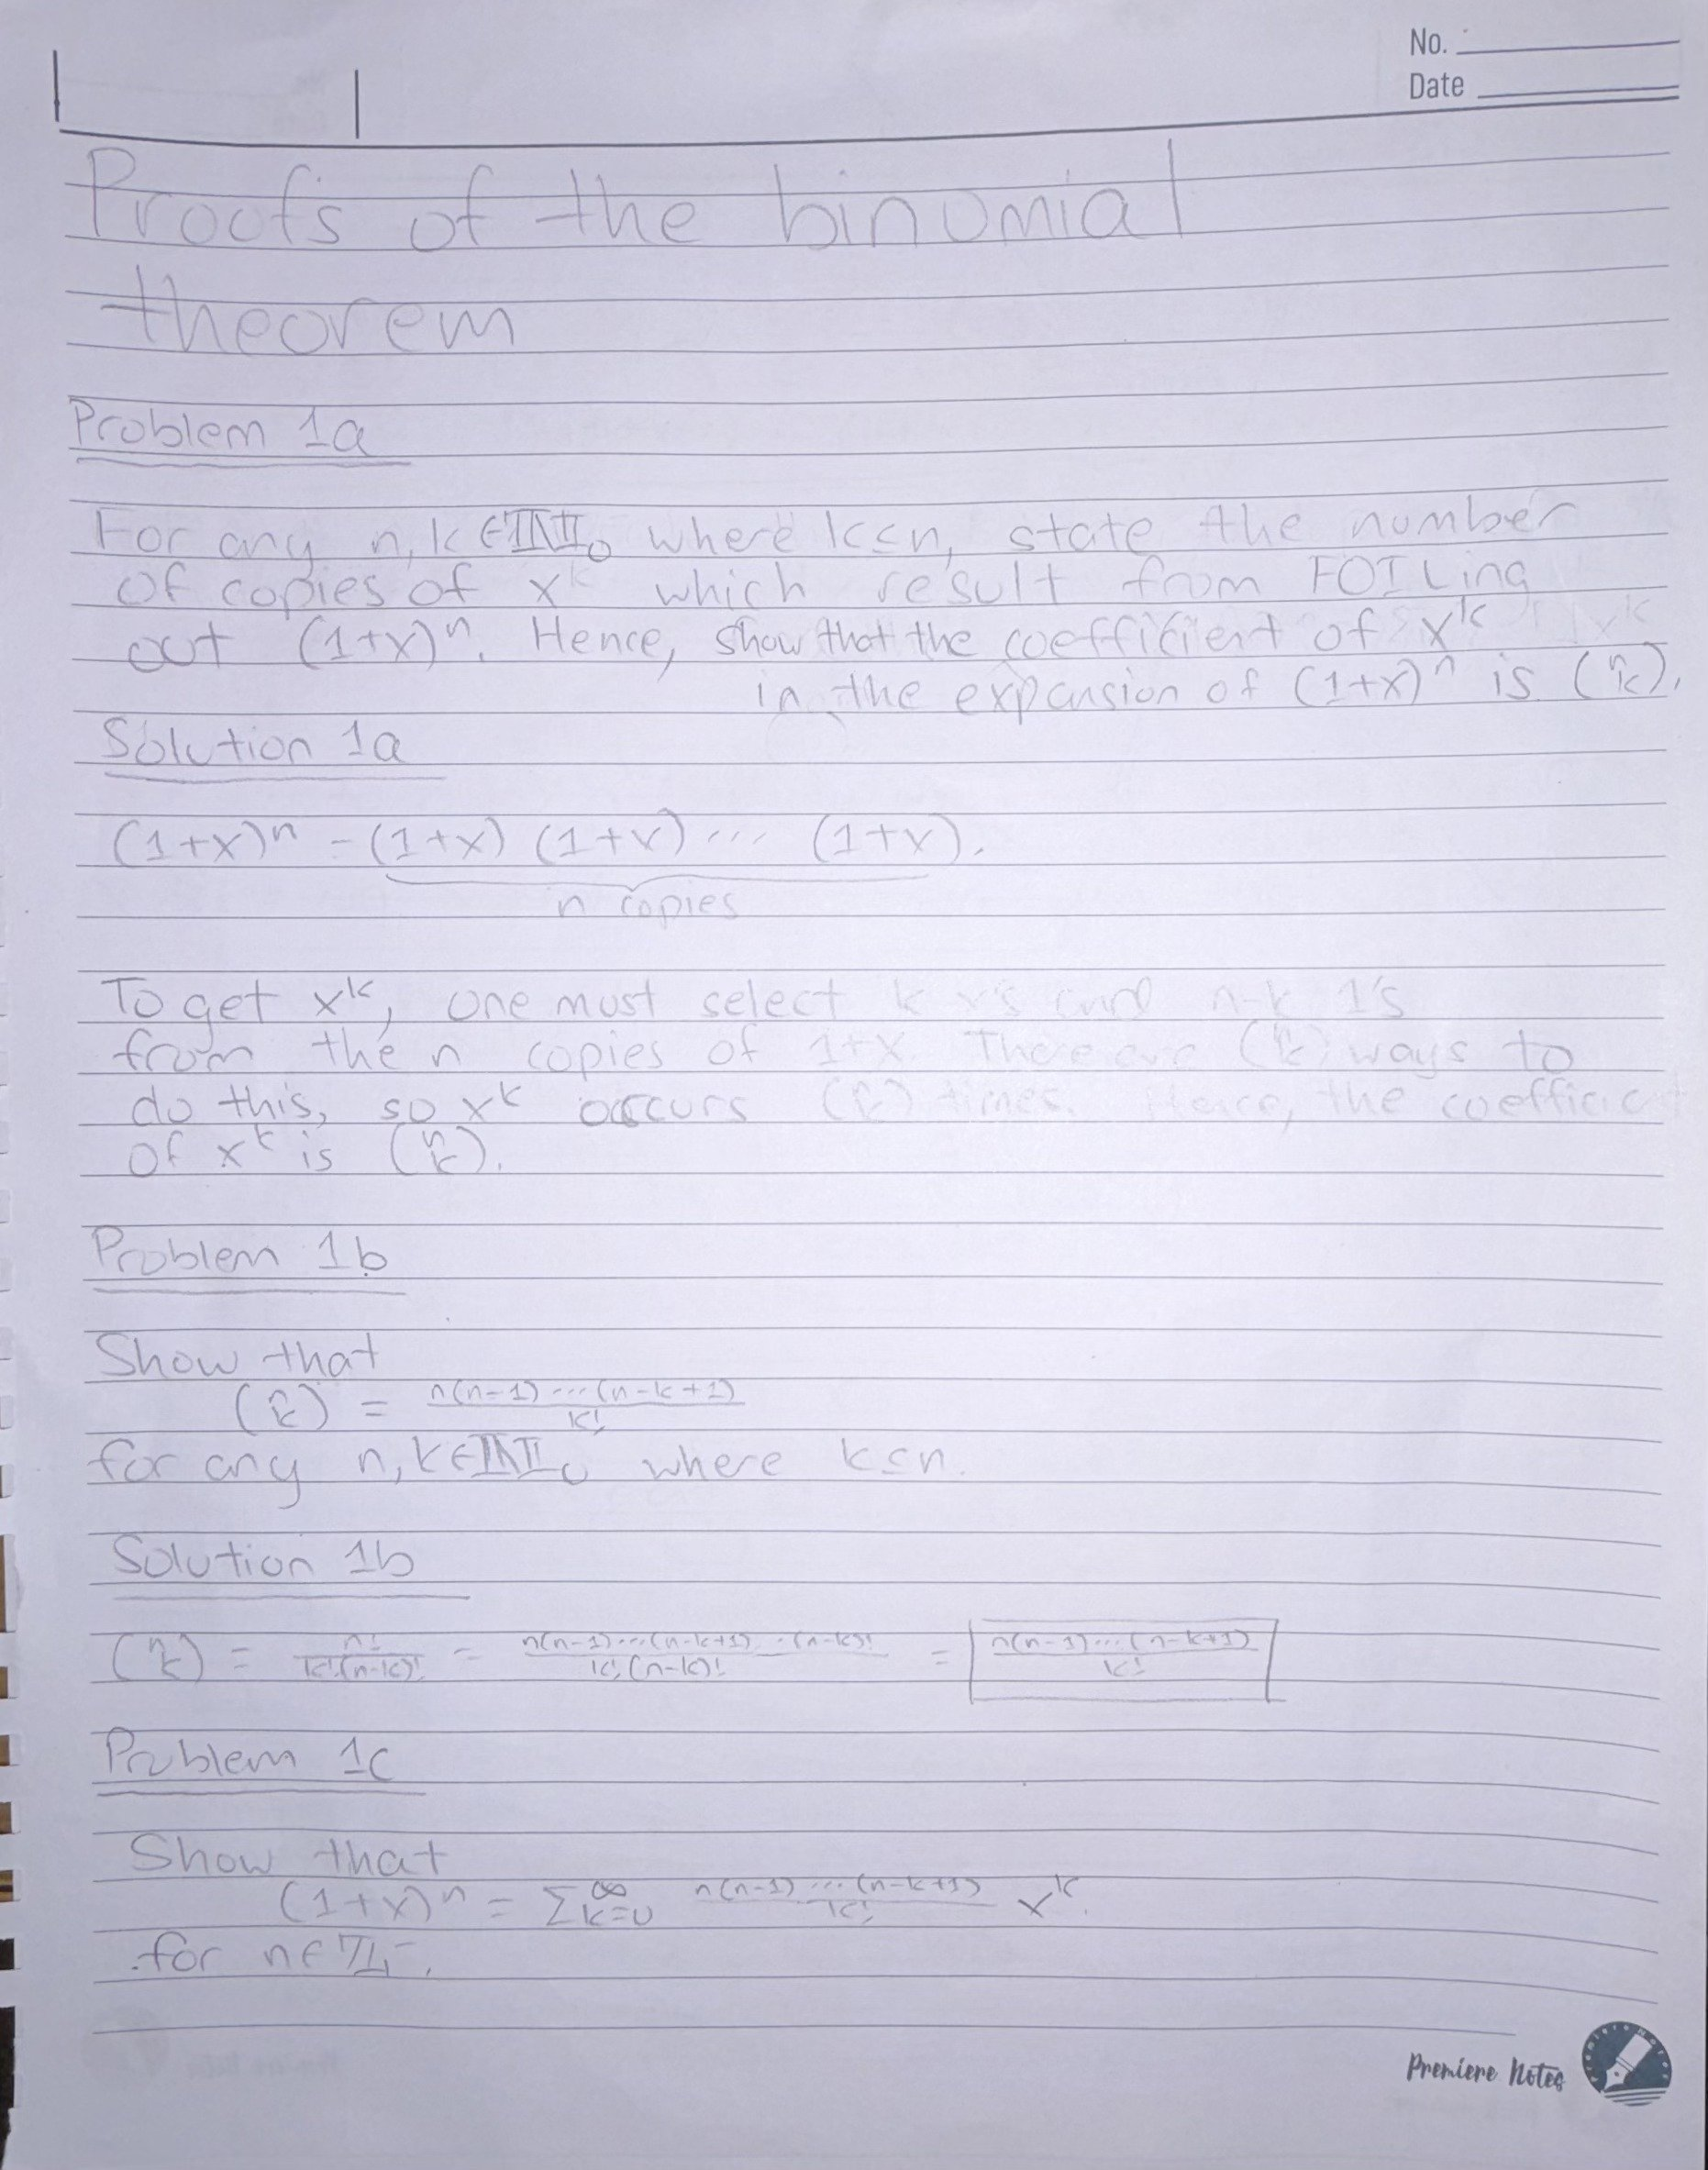
\includegraphics[width=0.48\textwidth]{figures/p1-page-1.jpg}
    \hfill
    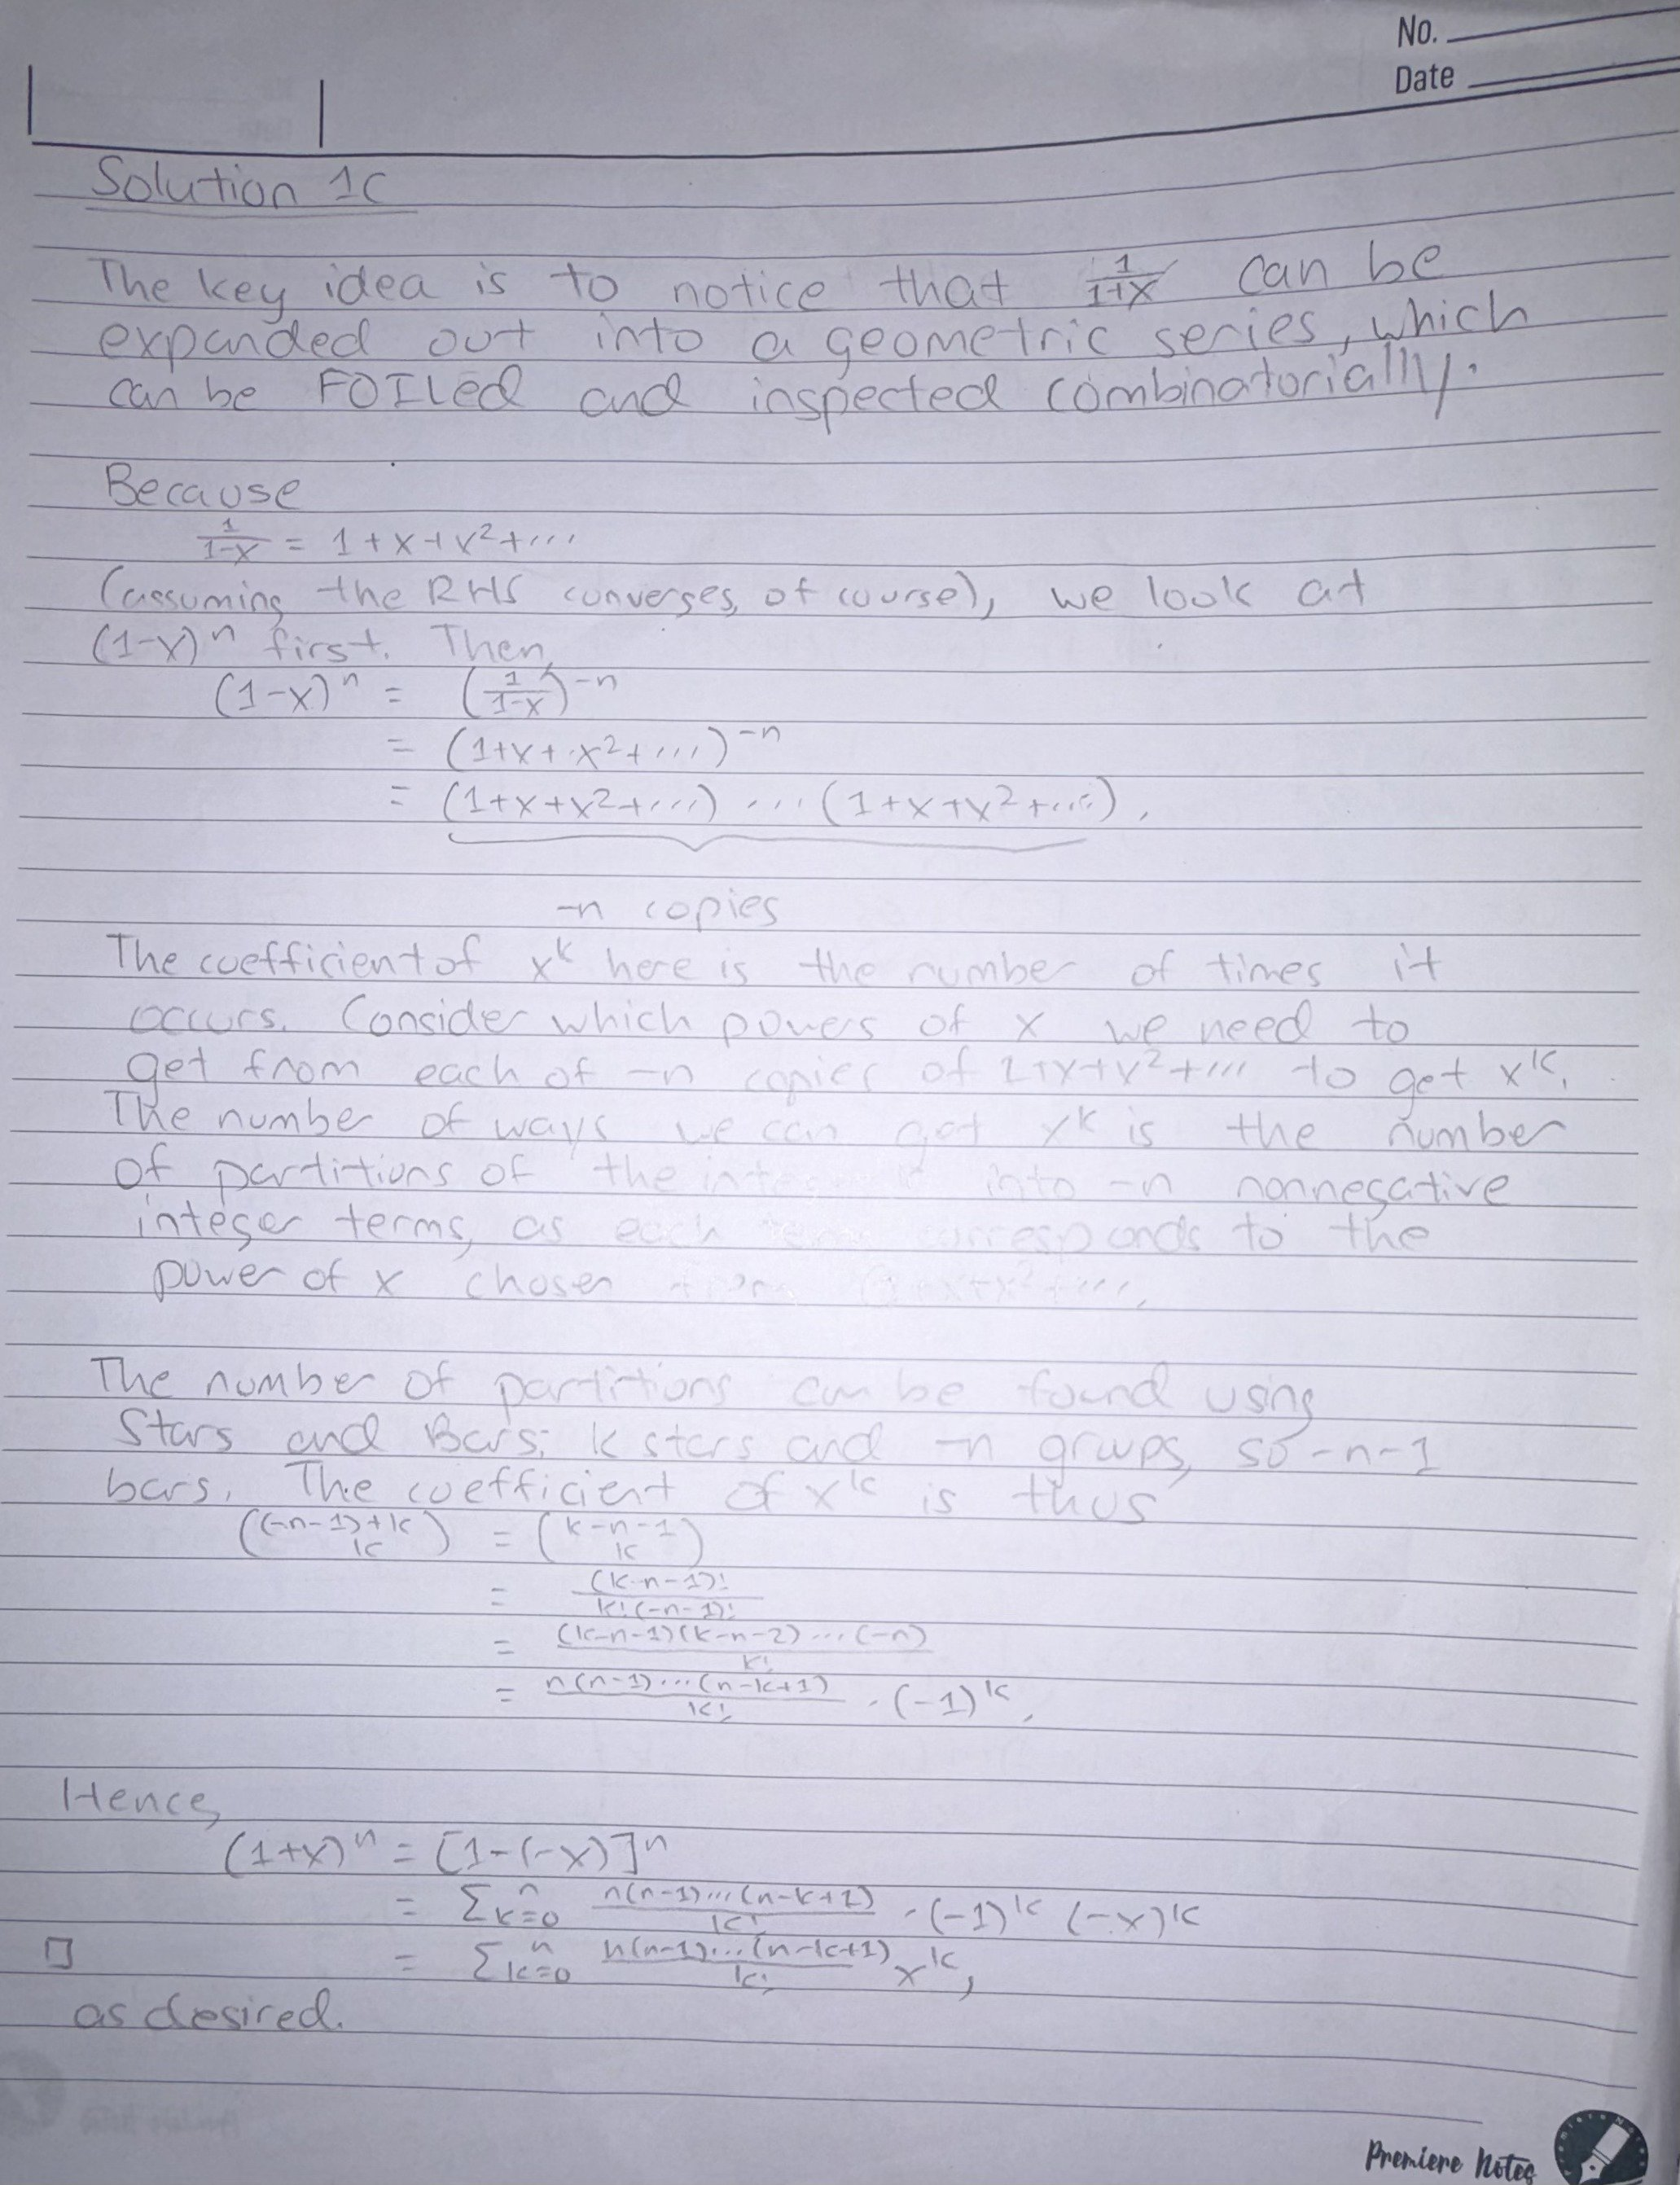
\includegraphics[width=0.48\textwidth]{figures/p2-page-1.jpg}
\end{figure}

\subsection{Problem 3}

\begin{figure}[H]
    \centering
    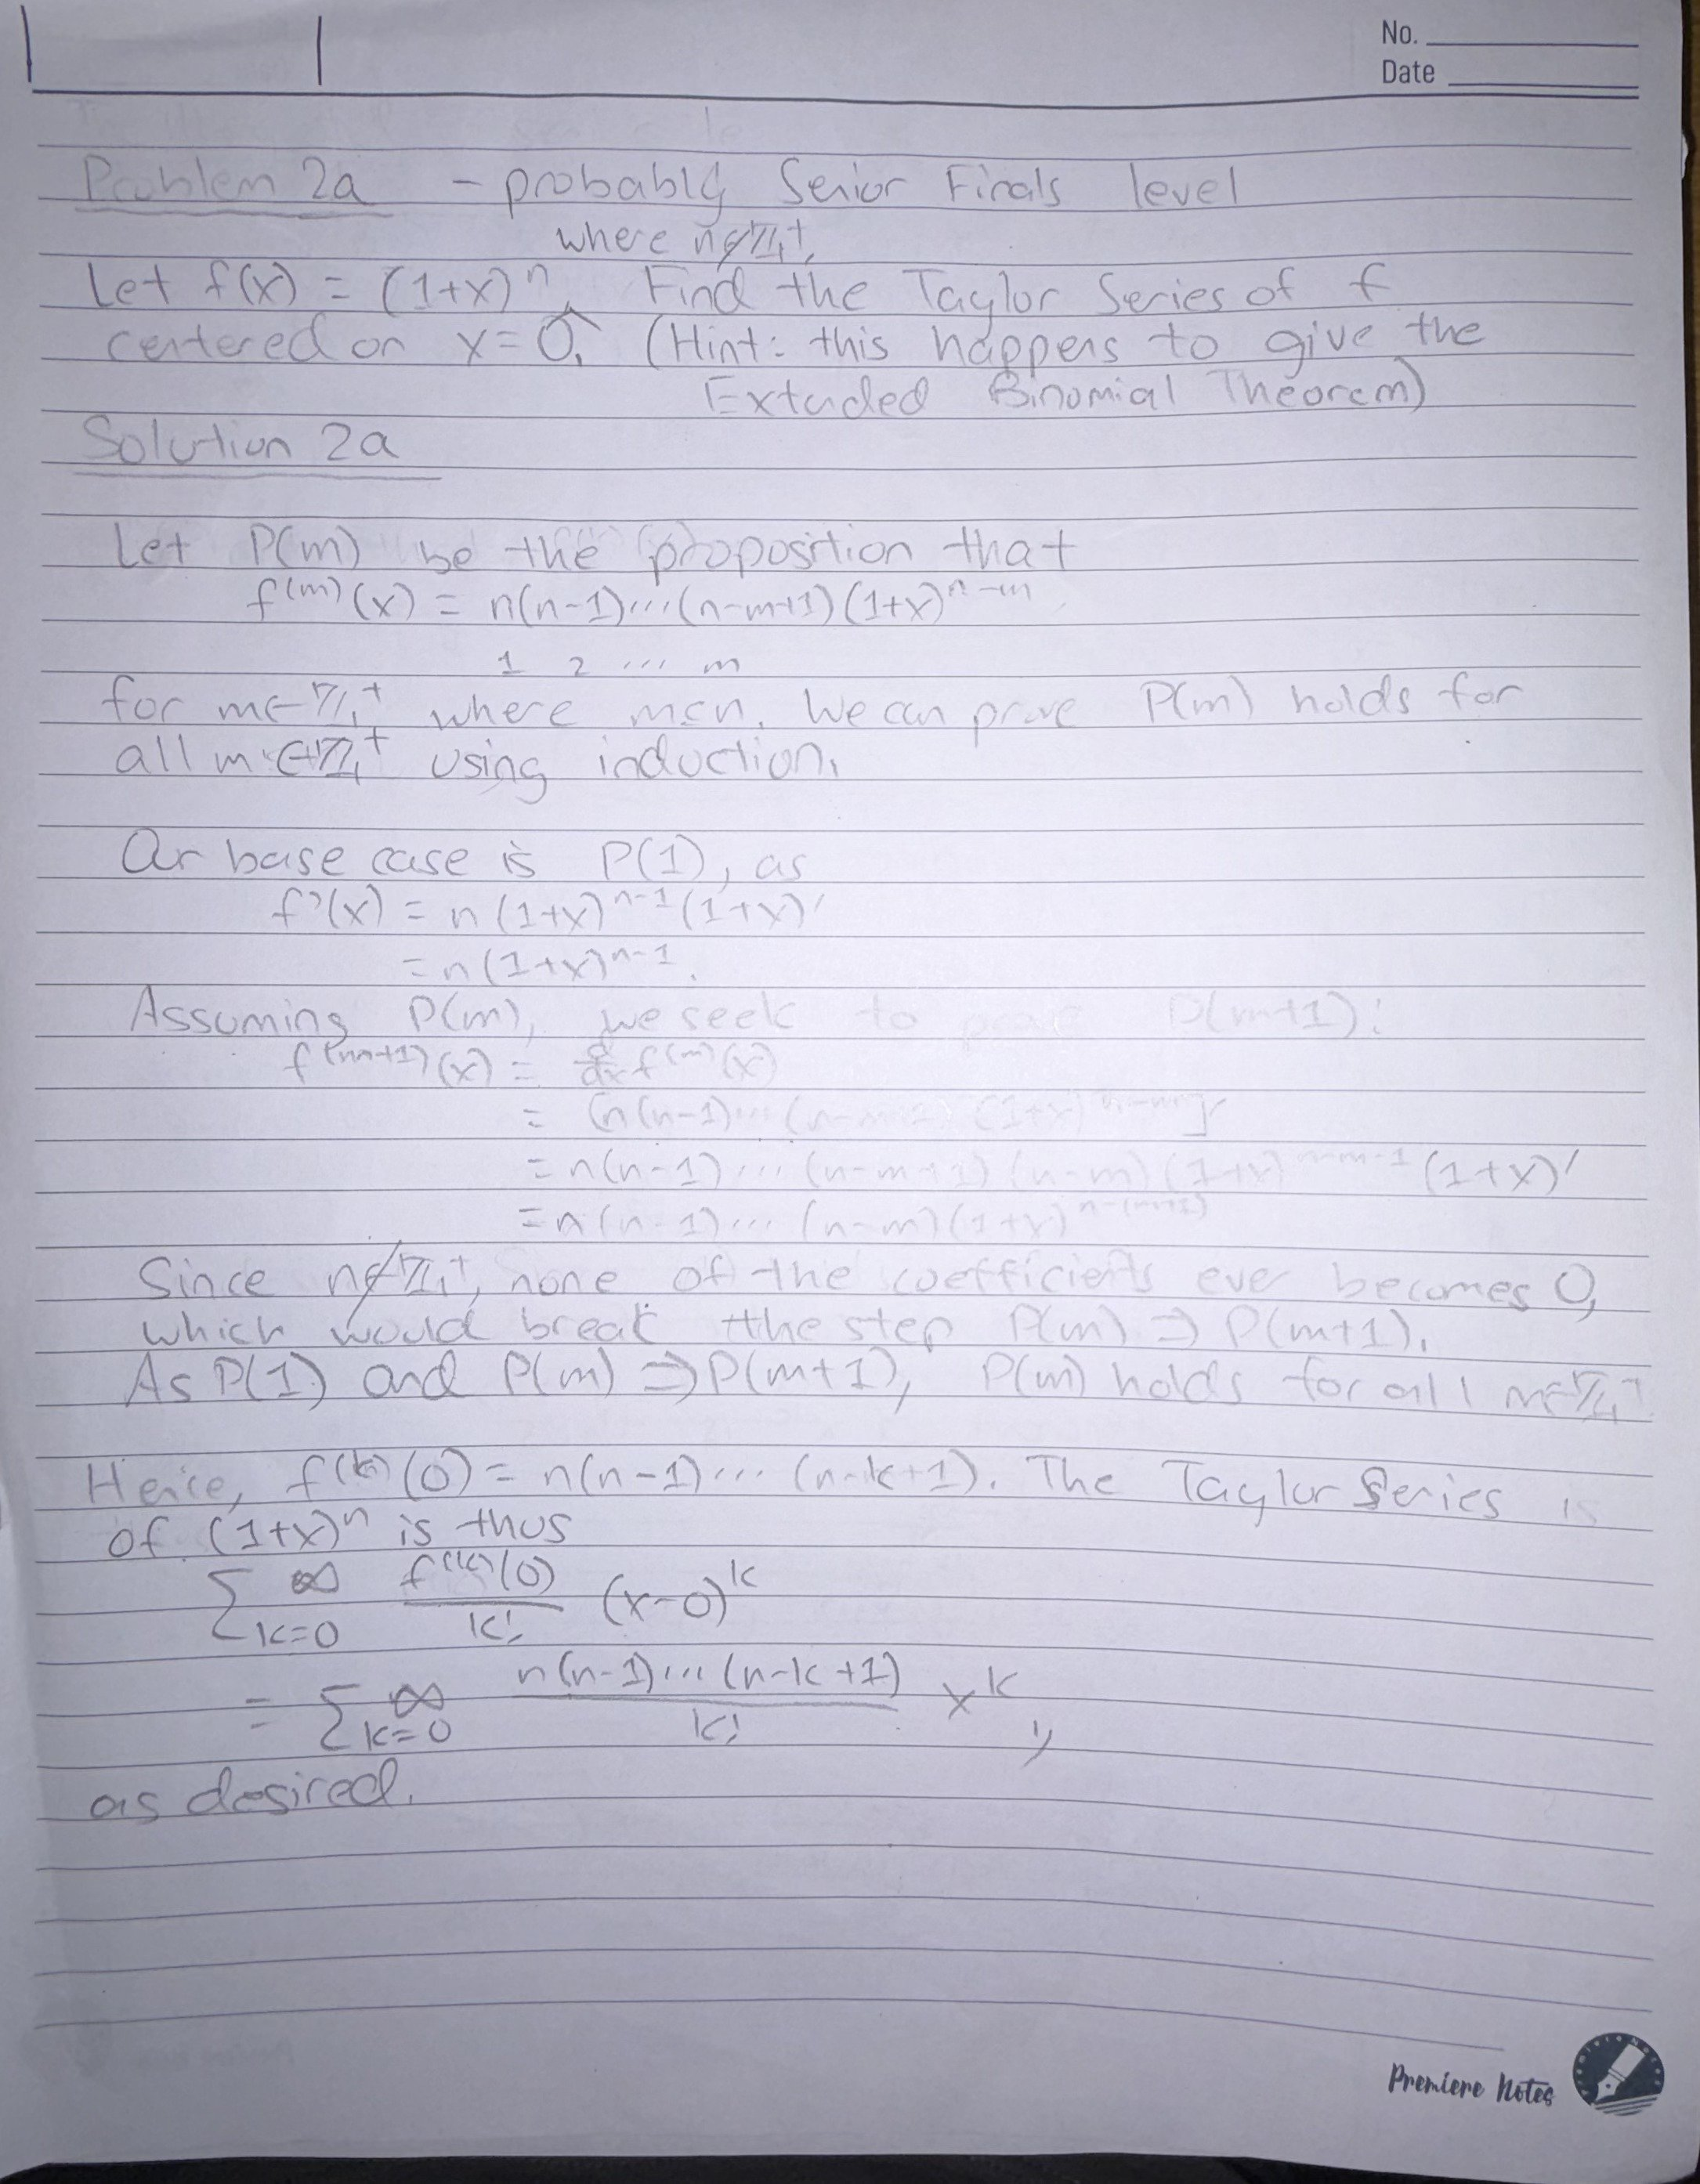
\includegraphics[width=0.48\textwidth]{figures/p3-page-1.jpg}
    \hfill
    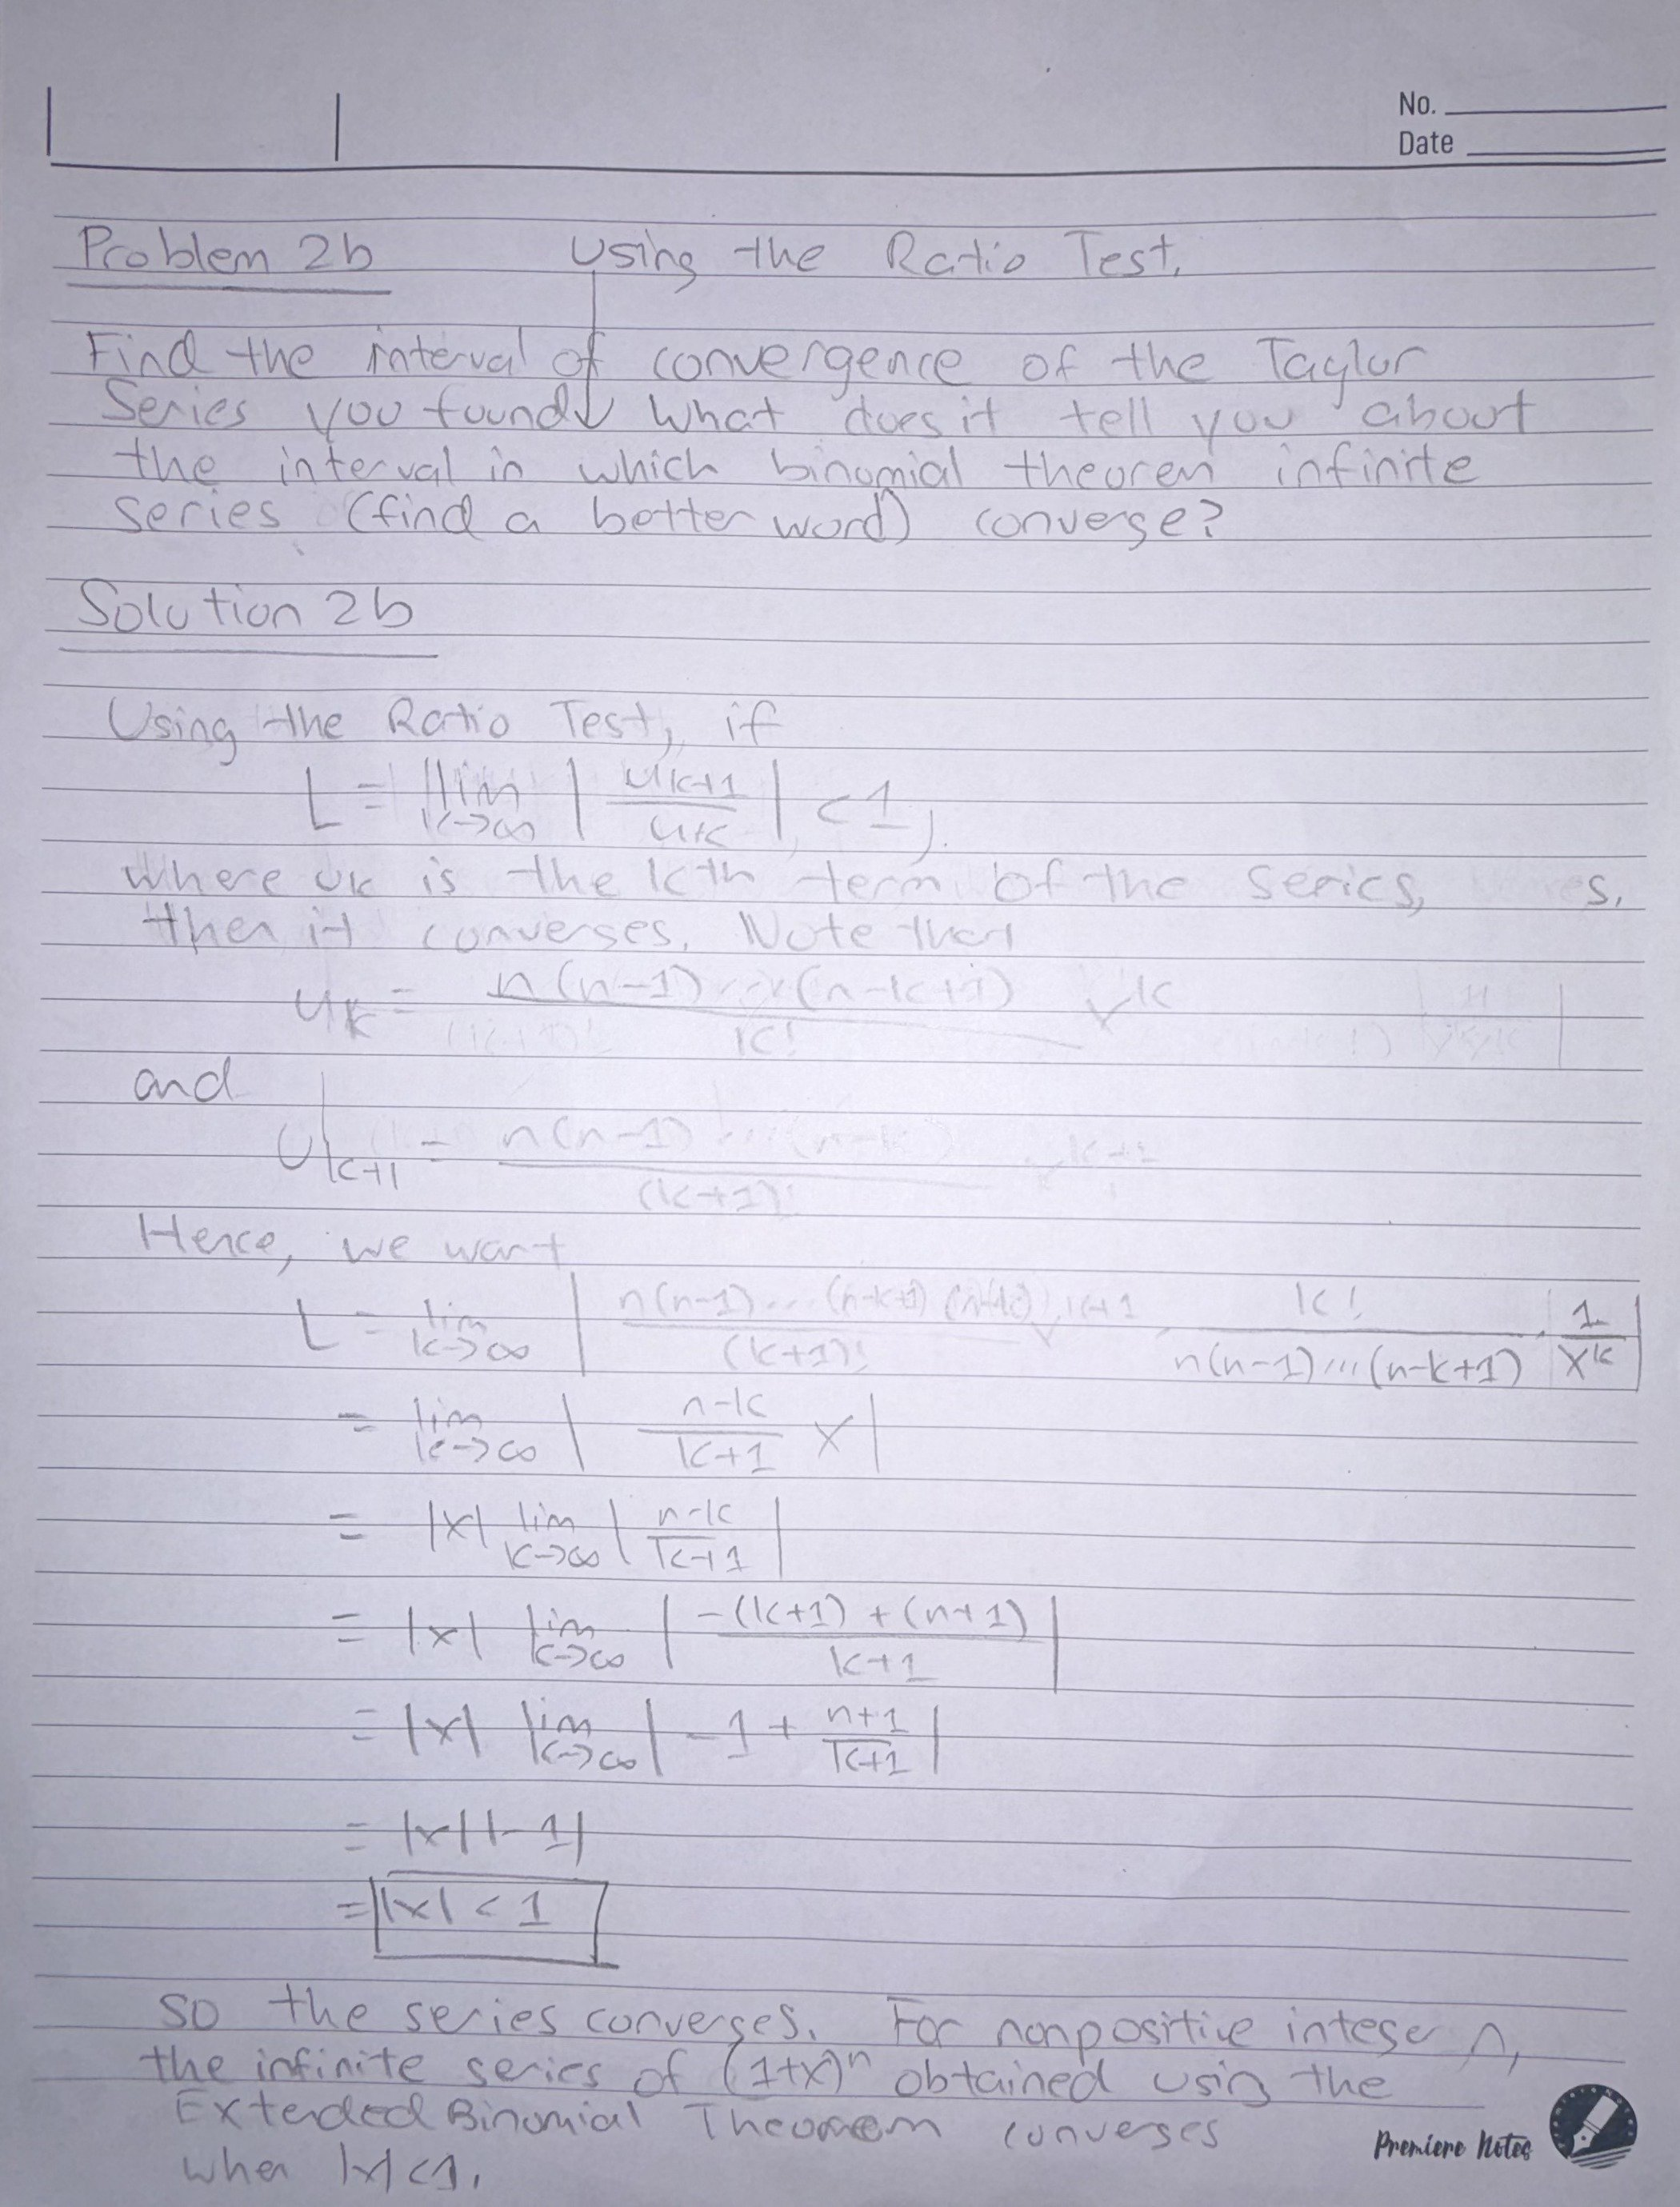
\includegraphics[width=0.48\textwidth]{figures/p3-page-2.jpg}
\end{figure}

\end{document}
